% ++++++++++++++++++++++++++++++++++++++++
% Don't modify this section unless you know what you're doing!
\documentclass[letterpaper,12pt]{article}
\usepackage{tabularx} % extra features for tabular environment
\usepackage{amsmath}  % improve math presentation
\usepackage{graphicx} % takes care of graphic including machinery
\usepackage[margin=0.75in,letterpaper]{geometry} % decreases margins
\usepackage{cite} % takes care of citations
\usepackage[final]{hyperref} % adds hyper links inside the generated pdf file
\usepackage{listings}
\usepackage{csvsimple}
\usepackage{verbatim}
\usepackage{float}
\usepackage{graphicx} % Allows including images
\hypersetup{
	colorlinks=true,       % false: boxed links; true: colored links
	linkcolor=black,        % color of internal links
	citecolor=blue,        % color of links to bibliography
	filecolor=magenta,     % color of file links
	urlcolor=blue         
}
%++++++++++++++++++++++++++++++++++++++++
\setlength{\parindent}{0pt}
\setlength\parskip{1em plus 0.1em minus 0.2em}

\begin{document}
\title{%
Electron Spin Resonance \\
\large PHY224 Lab 6}
\author{Fredrik Dahl Bråten, Pankaj Patil}
\date{\today}
\maketitle
%\tableofcontents
%\listoffigures
%\listoftables

\section{Abstract}

In this exercise we experimentally calculate the gyromagnetic ratio $\gamma$ for an electron. 
As we expect the ratio to be greater than the theoretically predicted value of $e/2m$, 
we compute this discrepancy in terms of \emph{Lande g factor}. This analysis was done in Python by use of the numpy, scipy and matplotlib modules.

\section{Introduction}


\section{Methods, Materials and Experimental Procedure}

We successfully followed the procedures as described by the TA and lab manual \cite{lab-manual-ex6} for this experiment.

\section{Results}

\section{Discussion}

\section{Conclusions}

\pagebreak

\appendix

\section{Appendix}

\subsection{Plots Frequency vs Magnetic Field}
\begin{figure}[H]
  \centering
  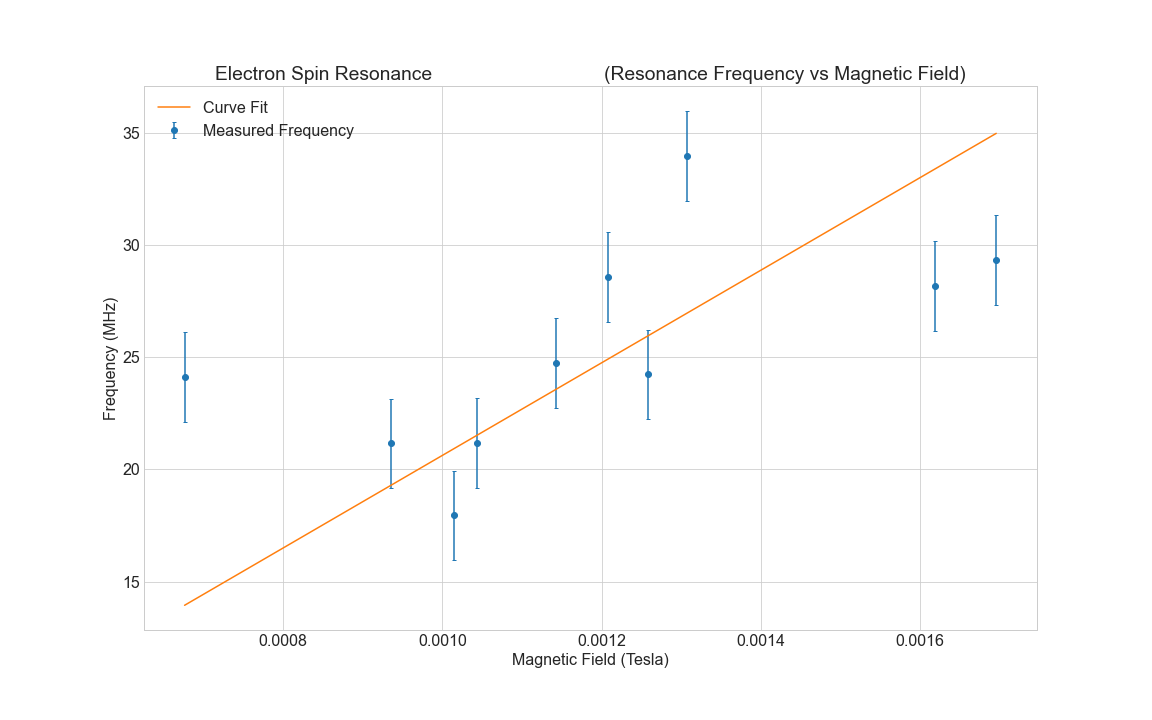
\includegraphics[width=0.95\linewidth]{../code/Pankaj/lab6_freq_vs_magnetic_field.png}    
  \begin{center}
    \begin{center}   
    \end{center}  \end{center}
  \caption{Frequency vs Magnetic Field}
  \label{frq-vs-b}
\end{figure}

\pagebreak

\subsection{Python Code}

\pagebreak

\begin{thebibliography}{99}

\bibitem{lab-manual-ex6} Electron Spin Resonance - electric-spin.pdf.pdf

\end{thebibliography}

\end{document}
